\chapter{Система имитационного моделирования.}

\section{Архитектура подсистемы имитационного моделирования}

В данном разделе будут рассмотрено внутренние устройство элемента архитектуры ПО (\ref{ris:arh1}), отвечающего за имитационное моделирование. 
Работа имитационной модели состоит из следующих этапов:

\begin{enumerate}
    \item[\mylabel{itm:point1}{1})] Создание шаблона продуктов. Шаблон представляет из себя структуру данных, являющийся отображением технологической карты одной единицы продукции.
	\item[\mylabel{itm:point2}{2})] Создание заказа. Заказ представляет из себя список структур данных, включающим в себя шаблон продукта и необходимое количество.
	\item[\mylabel{itm:point3}{3})] Следующим этапом является развертывание единого плана на основе заказа. Производственный план описывает совокупность операций\footnote{Так как технологическая карта описывается набором операций, а заказ описывается перечнем технологических карт и их количеством, появилась возможность описать план совокупностью операций.} и состояние ресурсов.
    \item[\mylabel{itm:point4}{4})] Пошаговая реализация плана с учетом ресурсных ограничений, где каждый раз при расчете операции обновляется информации о состоянии ресурсов.
\end{enumerate}

Работа имитационного моделирования представлена на рисунке \ref{ris:alg}
\begin{figure}[H]
    \center{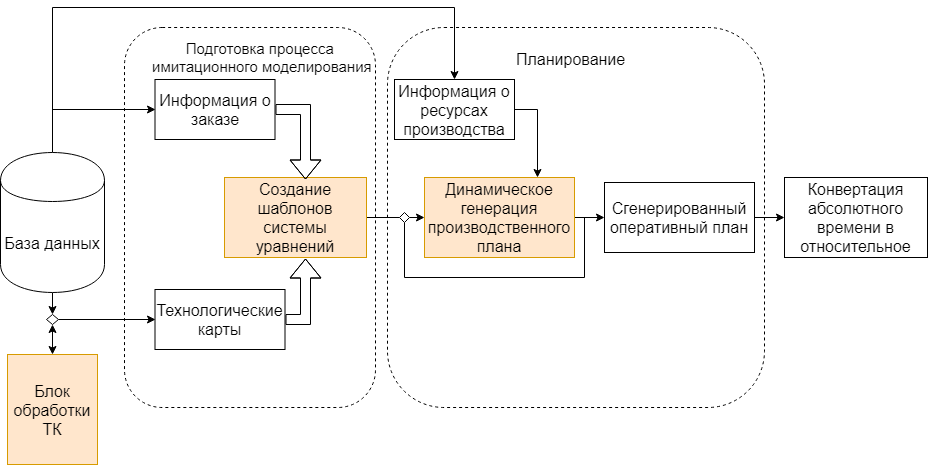
\includegraphics[width=1\linewidth]{fig/alg_2.png}}
    \caption{Визуализация работы имитационного моделирования}
    \label{ris:alg}
\end{figure}

\section{Входные и выходные данные}

\subsection{Входные данные}
В данном разделе приведены входные данные для имитационной модели. Благодаря модульности данного элемента ПО, в перечень включены данные не учтенные в текущей реализации, добавление данных планируется в будущем. Эти данные \textit{помечены курсивом}.

\begin{itemize}
	\item ЦПВ - цеховая последовательность выпуска (выпуск продукции осуществляется в порядке, в котором они записаны в ЦПВ):
		\begin{itemize}
			\item[а)] наименование продукции;
			\item[б)] количество единиц продукции;	
			\item[в)] технологическая карта.
		\end{itemize}			
	\item Технологические карты, подробнее смотри (\ref{assembly_line_balancing:input_data}).
	\item Производственные ресурсы;
	\item \textit{Трафик доступности ресурсов};
	\item \textit{Структура цеха};
	\item \textit{Минимальное время участия ресурса в операции};
	\item \textit{Штрафы за переключение ресурса с одной операции на другую}. 
\end{itemize}

\subsection{Выходные данные}

\begin{itemize}
	\item Расчетные данные:	
		\begin{itemize}
			\item[а)] перечень всех операций для всех единиц продукции ЦПВ;
			\item[б)] время начала всех операций;
			\item[в)] время окончания всех операций;
			\item[г)] \textit{производственные ресурсы, привлекаемые к выполнению операции};
			\item[д)] \textit{время начала и конца участия ресурса в операции};
			\item[е)] \textit{загрузка производственных ресурсов}.
		\end{itemize}		
	\item Визуализация данных пользователю:
		\begin{itemize}
			\item[а)] расписания для производственных ресурсов;
			\item[б)] диаграммы Ганта выпуска разных видов продукции;
			\item[в)] визуализация загрузки производственных ресурсов.
		\end{itemize}		 
\end{itemize}

\section{Этапы имитационного моделирования}
В данном разделе подробно описаны все этапы имитационного моделирования.
На изображении (\ref{ris:DataFlow}) приведена диаграмма потоков данных.

\begin{figure}[H]
    \center{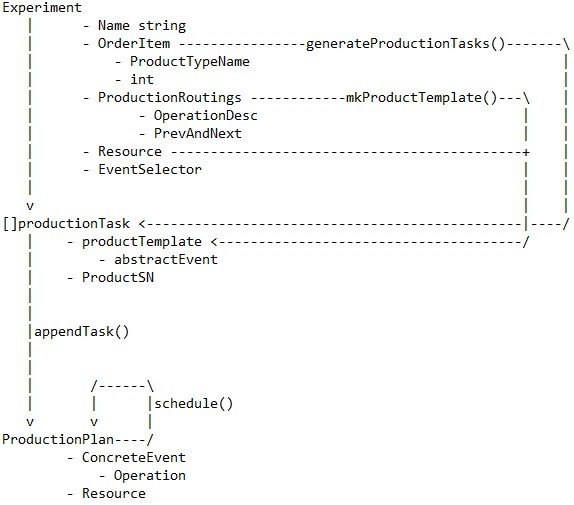
\includegraphics[width=1\linewidth]{fig/MkExperimentDataFLow.jpg}}
    \caption{Data flow imcore}
    \label{ris:DataFlow}
\end{figure}

\subsection{Предобработка технологических карт}

\subsubsection*{Входные данные}
\indent Входными данными для данного элемента ПО является технологическая карта с конфигурациями ресурсов\footnote{Примером конфигурации ресурса может являться вычисление длительности операции на основе количества персонала, привязанного к операции.}. 

\subsubsection*{Выходные данные}
Выходными данными являются технологическая карта с зафиксированными значениями.

\subsubsection*{Процесс предобработки}
\label{prepeocess}
Одним из первых этапов работы алгоритма имитационного моделирования является подготовка входных данных, полученных из базы данных. 

На текущий момент реализована небольшая часть функционала отвечающую за предварительную обработку. Одной из таких функций является расчет длительности операций. Так как длительность операций является переменной величиной, зависимой от трудоемкости и количества людей выполняющих операцию, существует четыре настройки ресурса:

\begin{enumerate}
    \item[1)] минимальная, при этом на операцию назначается минимальное количество людей, отсюда и длительность операции становится максимальной;
    \item[2)] максимальная, при этом на операцию назначается максимальное количество людей, отсюда и длительность операции становится минимальной;
    \item[3)] средняя при этом на операцию назначается среднее количество людей, отсюда и длительность операции становится средней;
    \item[4)] случайная, при этом количество персонала на операцию выбирается случайным образом. 
\end{enumerate}

Также одной из возможностей предварительной настройки является алгоритм выбора операции\footnote{В тех случаях, когда на этапе планирования есть независимые операции}. На данный момент существует две конфигурации:

\begin{itemize}
    \item[1)] стандартная, при которой выбор осуществляется строго по порядку расположения в структурах данных
    \item[2)] случайная, при этом случайным образом выбирается одна из возможных операций, которые доступны в данный момент 
\end{itemize}

Возможность менять входные данные являются важным этапом обработки входных данных полученных из базы данных, позволяя при этом подготовить данные для дальнейшей обработки, а также гибко менять параметризуемые величины, чем и достигается большая вариативность необходимая для поиска оптимального значения. 

\subsection{Создание шаблона продукта}

\subsubsection*{Входные данные}
Входными данными для данного элемента имитационной модели является технологическая карта с фиксированными значения (прошедшая обработку после базы данных).

\subsubsection*{Выходные данные}
\label{imcore:mkProductTemplate_output_data}
Выходными данными являются структура данных, включающая в себя набор событий и привязок ресурсов к каждому событию.

\subsubsection*{Описание реализации}
Для начала необходимо определить для чего нужны события. Как говорилось ранее любая технологическая карта состоит из перечня операций. В процессе работы было принято решение разделить операцию на события. Операция определяется двумя событиями: началом и концом. Такое разделение не случайно и вызвано необходимостью раздельной работы с началом и концом операций. Примером, когда это необходимо, является занятие и освобождение ресурса предприятия. При начальном событии алгоритм учитывает, то что данная операция потребляет ресурсы, при этом основным индикатором является начальное состояние. При конченом событии, когда ресурсы на операции использованы, происходит процесс высвобождения ресурсов, состояние ресурсов обновляется.

Основной задачей процесса создания шаблона продукта является подготовка необходимых структур данных для дальнейшей работы имитационной модели. На диаграмме потоков данных (\ref{ris:DataFlow}) данный процесс именуется, как - mkProductTemplate(). В результате работы, mkProductTemplate() создает шаблон продукта необходимый для структуры описывающий заказ.

\subsection{Создание заказа}

\subsubsection*{Входные данные}
Входными данными является перечень продуктов и количество каждого продукта из этого перечня.

\label{imcore:generateProductionTasks_output_data}

\subsubsection*{Выходные данные}
Выходными данными является список структур описываемых в разделе \ref{imcore:mkProductTemplate_output_data}, то есть шаблон и количество данного продукта.

\subsubsection*{Описание реализации}
На диаграмме потоков данных \ref{ris:DataFlow} процесс создания заказа называется - generateProductionTasks(). Основной задачей функции заказа является генерация шаблонов продуктов в зависимости от их количества, при этом каждый однотипный шаблон имеет уникальный идентификатор (серийный номер).


\subsection{Планирование}

\subsubsection*{Входные данные}
Входными данными для функции планирования является производственное задание на одну единицу продукции, полученное из списка сформировавшемся на этапе создания заказа (\ref{imcore:generateProductionTasks_output_data}).

\subsubsection*{Выходные данные}
Выходными данными является производственный план, состоящий из событий, операций и состояния ресурсов.

\subsubsection*{Описание реализации}
Основной задачей этапа планирования заключается в составлении плана, согласно которому выполняется привязка каждой операции для каждой единицы продукции к временным интервалам, конкретному работнику и конкретным производственным средствам. 
Результирующая блок-схема подсистемы имитационного моделирования изображена на рисунке \ref{ris:IM_blockShema}.

\begin{figure}[H]
    \center{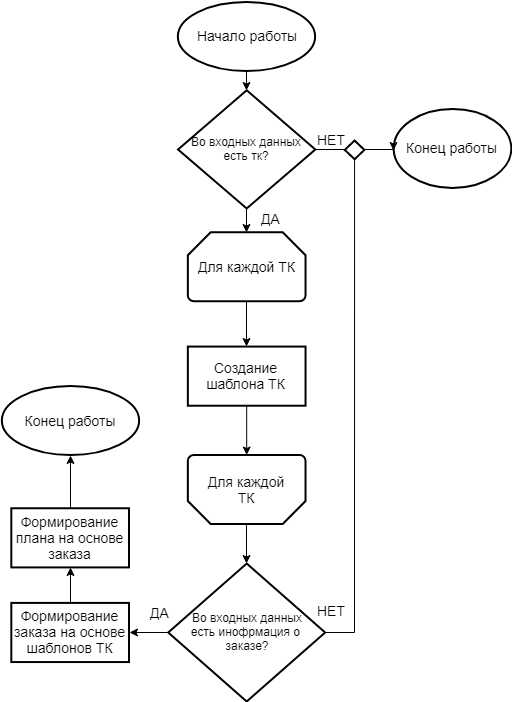
\includegraphics[scale=0.55]{fig/BlockShemaImcore.png}}
    \caption{Схема работы ядра имитационного моделирования}
    \label{ris:IM_blockShema}
\end{figure}


\subsection{Алгоритм модели ресурсов}

\indent В процессе создания оперативного плана, для получения корректной оценки времени выполнения операции или набора операций СПП необходимо ввести систему ограничений, которая будет отражать как ресурс, участвующий в операции может влиять на её время выполнения.
Это привело к созданию модели ресурсов накладывающей ограничения на выбор операции для расчета ядром имитационного моделирования.
Под ресурсом подразумевается любое устройство,деталь,инструмент или средство,за исключением сырьевого материала и промежуточного продукта, находящиеся в распоряжении предприятия для производства товаров и услуг.
В соответствии с данным определением к ресурсам относятся в том числе и человеческие ресурсы, которые в данной системе не рассматриваются с точки зрения поведения или других аспектов человеческой жизни, а лишь с точки зрения возможности выполнить конкретную задачу.
Также необходимо обозначить, что в данном разделе под моделью ресурса будет пониматься упрощенная модель реального ресурса, отражающая его основные (в рамках выполняемых операций) характеристики.\\
\indent Каждая модель ресурса представляет из себя структуру данных, которая должна реализовывать три метода:
\begin{itemize}
	\item метод привязки операции к модели ресурса;
	\item метод, осуществляющий проверку возможности выполнения данной операции моделью ресурса;
	\item метод, осуществляющий логику работы и в котором происходит изменение состояния данной модели.
\end{itemize}

\indent Под привязкой операции к модели подразумевается добавление операции в очередь на выполнение и, если это первая привязанная для данного продукта операция, то добавление продукта в очередь на распределение. Привязка осуществляется в начале работы системы, что позволяет ресурсам манипулировать ядром имитационного моделирования разрешая или запрещая выбирать привязанные к ним операции для расчета, что может повлечь за собой изменение последовательности выполнения операций и, соответственно, расчетного времени выполнения карты технологического процесса.

\begin{figure}[h]
	\centering
	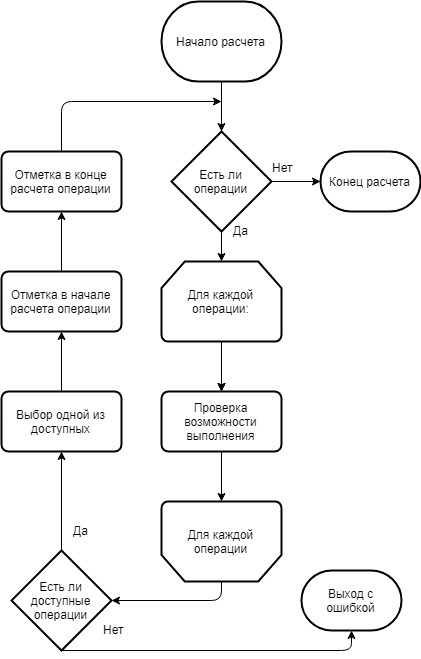
\includegraphics[scale=0.6]{fig/assemblyResSchema.png}
	\caption{Схема работы ядра моделирования с ресурсами в процессе расчета оперативного плана}
	\label{fig:assemblyResSchema}
\end{figure}

\indent Проверка производится во время работы системы и именно здесь происходит отбор операций в соответствии с внутренним состоянием модели.\\
\indent Логика осуществляется при выборке операции ядром и для каждой вызывается два раза: чтобы отметить состояние модели в начале и в конце расчета операции (см. \ref{fig:assemblyResSchema}).


% СПП имеет несколько видов ресурса, одним из которых является модель ресурса рабочих. Задача данной модели заключается в учете занятости каждого работника. Для упрощения работы модели было принято объединить группы работников одной   
\subsection{Оптимизация на уровне имитационного моделирования}

Как упоминалось ранее, в разделе посвященном предобработке технологической карты \ref{prepeocess}, исходная ТК предполагает вариативность конфигурации, отсюда следует, что потенциально имитационная модель может сгенерировать большое количество разных оперативных планов.

На рисунке \ref{ris:IM_process} приведена зависимость сгенерированного оперативного плана от выбранного критерия оптимальности.




\begin{figure}[H]
    \center{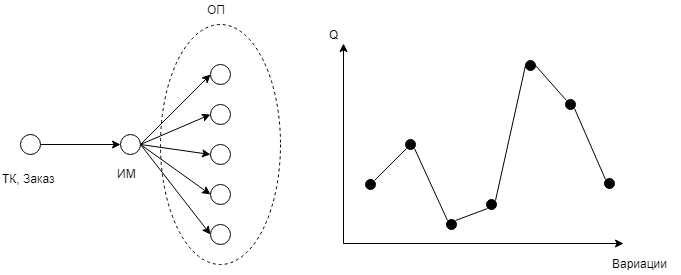
\includegraphics[width=1\linewidth]{fig/IM_process.png}}
    \caption{Процесс формирования оперативных планов и оценка их качества}
    \label{ris:IM_process}
\end{figure}

В следующем разделе приведены методы, которые позволяют подсистеме оптимизации (рис.\ref{ris:optimization}) на уровне имитационной модели, найти оптимальную последовательность операций. Критерием оптимальности в данном случае является минимальное время работы линии.

\begin{figure}[H]
    \center{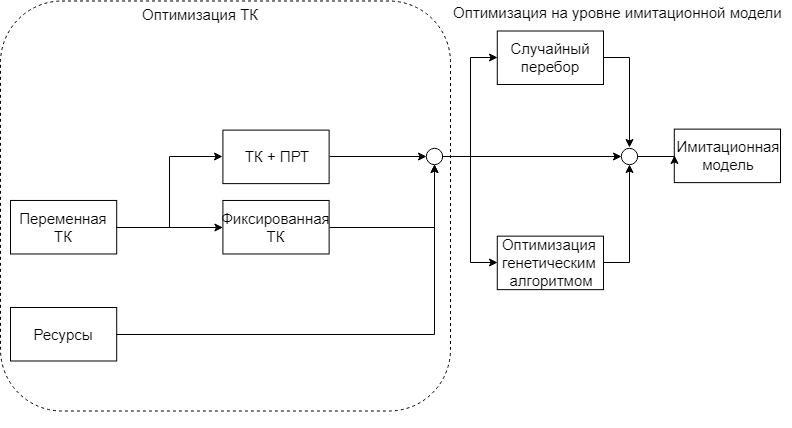
\includegraphics[width=1\linewidth]{fig/Opt.png}}
    \caption{Подсистема оптимизации}
    \label{ris:optimization}
\end{figure}


\subsubsection*{Метод случайного перебора}
Примером оптимизации может служить случайный выбор следующей операции при планировании, данный выбор возможен только в случаях одновременного выполнения нескольких независимых операций. Таким образом достигается вариативность при котором из разных реализаций, выбирается наилучший вариант. На рисунке \ref{ris:Force} изображены технологическая карта продукта и два плана, который были построены в результате случайного выбора операций.

\begin{figure}[H]
    \center{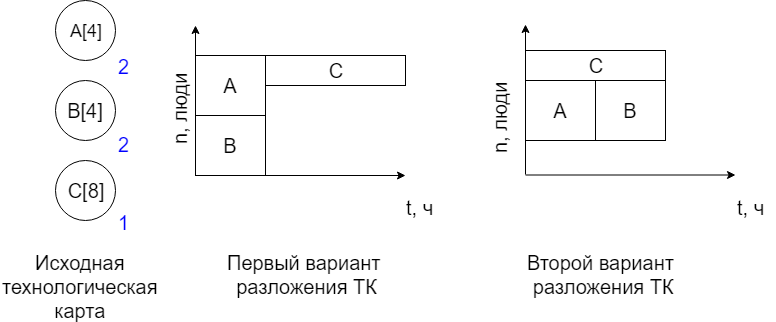
\includegraphics[width=1\linewidth]{fig/DecompositionOfTk.png}}
    \caption{Два плана, полученные путем перебора исходной технологической карты}
    \label{ris:Force}
\end{figure}

Пример на рисунке \ref{ris:Force} демонстрирует важность правильного выбора последовательности операций, обрабатываемой имитационной моделью. 

\subsubsection*{Генетические алгоритмы}
Основной задачей данного подхода является поиск оптимального значения путем смешивания и введения небольших правок (мутаций) в выборку наилучших решений.
Идеей такого рода алгоритмов является направленность поиска, которая позволяет преодолеть плато решений, при которых не происходит изменений в лучшую сторону. 


\section*{Эксперименты эффективности оптимизации}
\label{experiment}
Результаты экспериментов показали, что эффективность оптимизации во многом зависит от размера и состава входных данных.

Так на входных данных полученных от реального производства, оптимизация случайным перебором показала себя не эффективно. В первую очередь это связано с размером входных данных\footnote{325 операций в одной технологической карте.}. В вторых это связано со сложностью алгоритма планирования, так как сам случайный перебор является его частью, что делает его зависимым от реализации имитационной модели.

Также стоит отметить проблемы, связанные с входными данными. Данные проблемы заключаются в вариативности данных. На уровне имитационной модели метод случайного перебора может оперировать только выбором следующей операции на обработку. Таким образом, если операции на выбор только одна, в случае когда последовательность операций в технологической карте задана строгим образом и такая связь задана для большинства операций, то количество вариантов стремится к минимуму, а значит и целесообразность применения метода ставится под вопросом.

В результате эксперимента была сделаны следующие выводы. Метод случайного перебора зависит от размера входных данных, при этом важно оценивать входные данные на предмет вариативности. Также стоит отметить, что сложность задачи определяется пользователем на этапе конфигурации перебора\footnote{Имеется ввиду количество итераций случайного перебора.}, что еще сильнее повышает ценность предварительной оценки технологической карты.

\section{Результаты работы имитационной модели}

Проведение экспериментов над имитационной моделью показали следующие результаты.

Во первых при большом объеме входных данных имитационная модель работает не эффективно, что обусловлено исполнением алгоритмов, которые имеют большую вычислительную сложность.
Данная проблема частично решилась благодаря использованию возможностей языка программирования golang, при этом задача имитационного моделирования разделась на потоки, что позволяло одновременно обрабатывать несколько входных технологических карт.

Во вторых, выяснилось, что потенциально основной проблемой в будущем может оказаться доступность реальных данный для работы имитационной модели.
В рамках дипломной работы проверка имитационной модели проверялась на реальных технологических картах, при этом возник закономерный вопрос о сложности получения и организации данных о предприятии. 


Таким образом, задачу поставленную в рамках дипломной работы по созданию имитационной модели производственных процессов считаю выполненной. 
При этом возникли новые, связанные задачи, которые будут предметом для следующих исследований.